\documentclass{article}
\usepackage{amsmath}
\usepackage{graphicx}
\usepackage{float}

\title{AP Statistics Part 1 Practice}
\author{Rishi Salwi and Eric Zheng}

\begin{document}
\maketitle

\begin{enumerate}
  % Question 1
  % I'll organize all the plots once they're done
  \item The following plots were created:
    \begin{enumerate}
      \item Stem and leaf plot:
      \item Frequency table:
      \item Histogram:
        \begin{figure}[H]
          \centering
          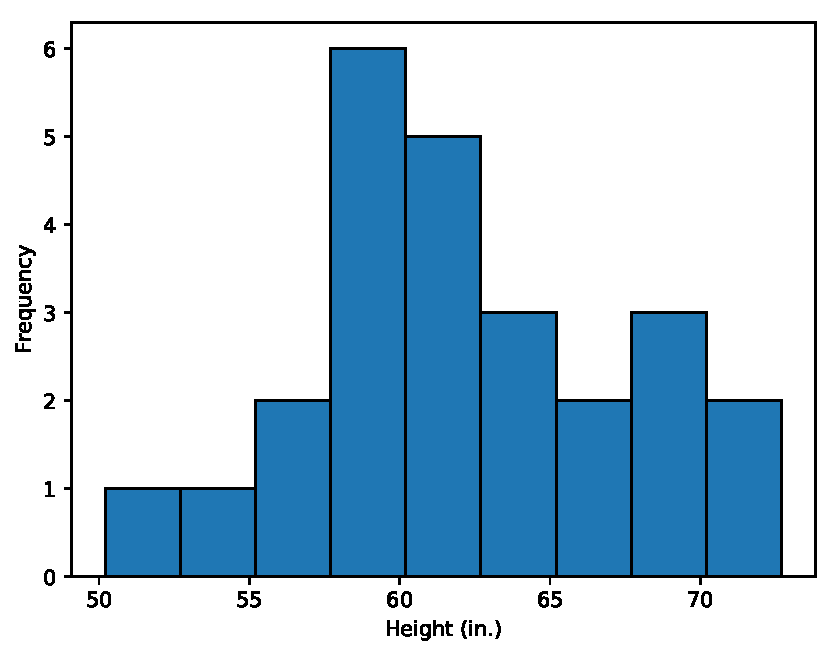
\includegraphics[width=\textwidth]{histogram.pdf}
          \caption{A histogram showing women's heights (in inches)}
        \end{figure}
      \item Pie chart:
        \begin{figure}[H]
          \centering
          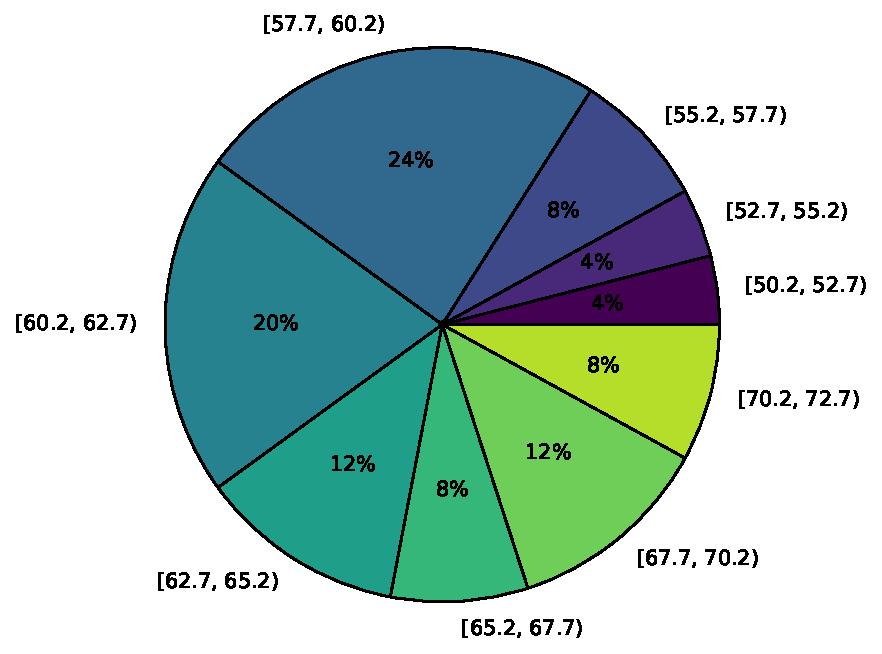
\includegraphics[width=\textwidth]{pie.pdf}
          \caption{A pie chart showing women's heights (in inches)}
        \end{figure}
      \item Box plot:
        \begin{figure}[H]
          \centering
          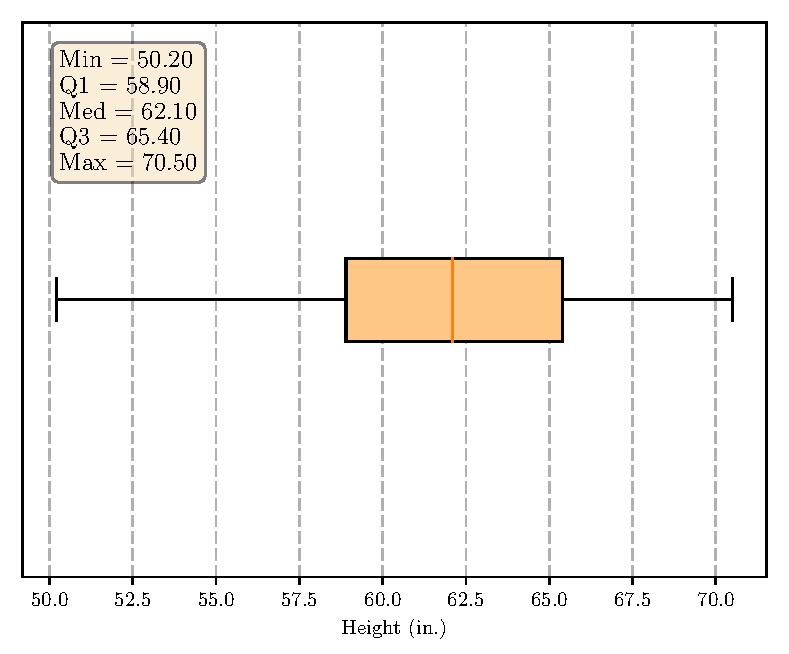
\includegraphics[width=\textwidth]{box.pdf}
          \caption{A box plot showing women's heights (in inches)}
        \end{figure}
    \end{enumerate}

  % Question 2
  \item These data were used to compute the following sample summative statistics:
    \begin{table}[H]
      \centering
      \caption{Summative statistics about women's heights (in inches)}
      \begin{tabular}{l c}
        \hline
        Statistic & Value \\
        \hline
        Mean & 61.88 \\
        Median & 62.1 \\
        Mode & 59.3, 62.1, 62.4, 63.1, 68.5 \\
        Midrange & 10.15 \\
        Range & 20.3 \\
        Variance & 25.68 \\
        Standard Deviation & 5.07 \\
        \hline
      \end{tabular}
    \end{table}

  % Question 3
  \item The data set is not normally distributed; this can be most easily seen from the shape of the histogram, which does not resemble a bell curve. It is not symmetric because it is skewed to the left. I know this because there is a whale tail.
\end{enumerate}
\end{document}
